\documentclass[10pt,oneside]{article}
\usepackage[T1]{fontenc}
\usepackage[utf8]{inputenc}
% \usepackage{lmodern}
%\usepackage[adobe-utopia,uppercase=upright,greeklowercase=upright]{mathdesign}
\usepackage[adobe-utopia]{mathdesign}
%\usepackage{minionpro}
% \usepackage{pifont}
% \usepackage{amssymb}
\usepackage{amsmath}
\usepackage[francais]{babel}
% \usepackage[francais]{varioref}
\usepackage[dvips]{graphicx}

\usepackage{framed}
\usepackage[normalem]{ulem}
\usepackage{fancyhdr}
\usepackage{titlesec}
\usepackage{vmargin}
\usepackage{longtable}

\usepackage{ifthen}


%\usepackage{epsfig}
\usepackage{subfig}

\usepackage{multirow}
\usepackage{multicol} % Portions de texte en colonnes
\usepackage{flafter}%floatants après la référence



\usepackage{color}
\usepackage{colortbl}


\definecolor{gris25}{gray}{0.75}
\definecolor{bleu}{RGB}{18,33,98}
\definecolor{bleuf}{RGB}{42,94,171}
\definecolor{bleuc}{RGB}{231,239,247}
\definecolor{rougef}{RGB}{185,18,27}
\definecolor{rougec}{RGB}{255,230,231}
\definecolor{vertf}{RGB}{103,126,82}
\definecolor{vertc}{RGB}{220,255,191}

\newenvironment{rem}[1][\hsize]%
{%
    \def\FrameCommand
    {%
\rotatebox{90}{\textit{\textsf{Remarque}}} 
        {\color{bleuf}\vrule width 3pt}%
        \hspace{0pt}%must no space.
        \fboxsep=\FrameSep\colorbox{bleuc}%
    }%
    \MakeFramed{\hsize#1\advance\hsize-\width\FrameRestore}%
}%
{\endMakeFramed}%


\newenvironment{savoir}[1][\hsize]%
{%
    \def\FrameCommand
    {%
\rotatebox{90}{\textit{\textsf{Savoir}}} 
        {\color{bleuf}\vrule width 3pt}%
        \hspace{0pt}%must no space.
        \fboxsep=\FrameSep\colorbox{bleuc}%
    }%
    \MakeFramed{\hsize#1\advance\hsize-\width\FrameRestore}%
}%
{\endMakeFramed}%

\newenvironment{prob}[1][\hsize]%
{%
    \def\FrameCommand%
    {%
\rotatebox{90}{\textit{\textsf{ Problématique}}} 
        {\color{rougef}\vrule width 3pt}%
        \hspace{0pt}%must no space.
        \fboxsep=\FrameSep\colorbox{rougec}%
    }%
    \MakeFramed{\hsize#1\advance\hsize-\width\FrameRestore}%
}%
{\endMakeFramed}%

\newenvironment{obj}[1][\hsize]%
{%
    \def\FrameCommand%
    {%
\rotatebox{90}{\textit{\textsf{ $\;$}}} 
        {\color{rougef}\vrule width 3pt}%
        \hspace{0pt}%must no space.
        \fboxsep=\FrameSep\colorbox{rougec}%
    }%
    \MakeFramed{\hsize#1\advance\hsize-\width\FrameRestore}%
}%
{\endMakeFramed}%

\newenvironment{defi}[1][\hsize]%
{%
    \def\FrameCommand%
    {%
\rotatebox{90}{\textit{\textsf{Définition\\}}} 
        {\color{bleuf}\vrule width 3pt}%
        \hspace{0pt}%must no space.
        \fboxsep=\FrameSep\colorbox{bleuc}%
    }%
    \MakeFramed{\hsize#1\advance\hsize-\width\FrameRestore}%
}%
{\endMakeFramed}%


\newenvironment{hypo}[1][\hsize]%
{%
    \def\FrameCommand%
    {%
\rotatebox{90}{\textit{\textsf{Hypothèse\\}}} 
        {\color{bleuf}\vrule width 3pt}%
        \hspace{0pt}%must no space.
        \fboxsep=\FrameSep\colorbox{bleuc}%
    }%
    \MakeFramed{\hsize#1\advance\hsize-\width\FrameRestore}%
}%
{\endMakeFramed}%


\newenvironment{prop}[1][\hsize]%
{%
    \def\FrameCommand%
    {%
\rotatebox{90}{\textit{\textsf{Propriété\\}}} 
        {\color{bleuf}\vrule width 3pt}%
        \hspace{0pt}%must no space.
        \fboxsep=\FrameSep\colorbox{bleuc}%
    }%
    \MakeFramed{\hsize#1\advance\hsize-\width\FrameRestore}%
}%
{\endMakeFramed}%

\newenvironment{props}[1][\hsize]%
{%
    \def\FrameCommand%
    {%
\rotatebox{90}{\textit{\textsf{Propriétés\\}}} 
        {\color{bleuf}\vrule width 3pt}%
        \hspace{0pt}%must no space.
        \fboxsep=\FrameSep\colorbox{bleuc}%
    }%
    \MakeFramed{\hsize#1\advance\hsize-\width\FrameRestore}%
}%
{\endMakeFramed}%

\newenvironment{exemple}[1][\hsize]%
{%
    \def\FrameCommand%
    {%
\rotatebox{90}{\textit{\textsf{Exemple\\}}} 
        {\color{vertf}\vrule width 3pt}%
        \hspace{0pt}%must no space.
        \fboxsep=\FrameSep\colorbox{vertc}%
    }%
    \MakeFramed{\hsize#1\advance\hsize-\width\FrameRestore}%
}%
{\endMakeFramed}%

\newenvironment{resultat}[1][\hsize]%
{%
    \def\FrameCommand%
    {%
\rotatebox{90}{\textit{\textsf{Résultat\\}}} 
        {\color{rougef}\vrule width 3pt}%
        \hspace{0pt}%must no space.
        \fboxsep=\FrameSep\colorbox{rougec}%
    }%
    \MakeFramed{\hsize#1\advance\hsize-\width\FrameRestore}%
}%
{\endMakeFramed}%

\newenvironment{methode}[1][\hsize]%
{%
    \def\FrameCommand%
    {%
\rotatebox{90}{\textit{\textsf{Méthode\\}}} 
        {\color{rougef}\vrule width 3pt}%
        \hspace{0pt}%must no space.
        \fboxsep=\FrameSep\colorbox{rougec}%
    }%
    \MakeFramed{\hsize#1\advance\hsize-\width\FrameRestore}%
}%
{\endMakeFramed}%

\newenvironment{theo}[1][\hsize]%
{%
    \def\FrameCommand%
    {%
\rotatebox{90}{\textit{\textsf{Théorème\\}}} 
        {\color{rougef}\vrule width 3pt}%
        \hspace{0pt}%must no space.
        \fboxsep=\FrameSep\colorbox{rougec}%
    }%
    \MakeFramed{\hsize#1\advance\hsize-\width\FrameRestore}%
}%
{\endMakeFramed}%

\newenvironment{warn}[1][\hsize]%
{%
    \def\FrameCommand%
    {%
\rotatebox{90}{\textit{\textsf{Attention\\}}} 
        {\color{rougef}\vrule width 3pt}%
        \hspace{0pt}%must no space.
        \fboxsep=\FrameSep\colorbox{rougec}%
    }%
    \MakeFramed{\hsize#1\advance\hsize-\width\FrameRestore}%
}%
{\endMakeFramed}%

% \usepackage{pstricks}
%\usepackage{minitoc}
% \setcounter{minitocdepth}{4}

\setcounter{tocdepth}{2}

% \mtcselectlanguage{french} 

%\usepackage{draftcopy}% "Brouillon"
% \usepackage{floatflt}
\usepackage{psfrag}
%\usepackage{listings} % Permet d'insérer du code de programmation
\renewcommand{\baselinestretch}{1.2}

% Changer la numérotation des figures :
% ------------------------------------
% \makeatletter
% \renewcommand{\thefigure}{\ifnum \c@section>\z@ \thesection.\fi
%  \@arabic\c@figure}
% \@addtoreset{figure}{section}
% \makeatother
 


%%%%%%%%%%%%
% Définition des vecteurs %
%%%%%%%%%%%%
 \newcommand{\vect}[1]{\overrightarrow{#1}}

%%%%%%%%%%%%
% Définition des torseusr %
%%%%%%%%%%%%

 \newcommand{\torseur}[1]{%
\left\{{#1}\right\}
}

\newcommand{\torseurcin}[3]{%
\left\{\mathcal{#1} \left(#2/#3 \right) \right\}
}

\newcommand{\torseurstat}[3]{%
\left\{\mathcal{#1} \left(#2\rightarrow #3 \right) \right\}
}

 \newcommand{\torseurc}[8]{%
%\left\{#1 \right\}=
\left\{
{#1}
\right\}
 = 
\left\{%
\begin{array}{cc}%
{#2} & {#5}\\%
{#3} & {#6}\\%
{#4} & {#7}\\%
\end{array}%
\right\}_{#8}%
}

 \newcommand{\torseurcol}[7]{
\left\{%
\begin{array}{cc}%
{#1} & {#4}\\%
{#2} & {#5}\\%
{#3} & {#6}\\%
\end{array}%
\right\}_{#7}%
}

 \newcommand{\torseurl}[3]{%
%\left\{\mathcal{#1}\right\}_{#2}=%
\left\{%
\begin{array}{l}%
{#1} \\%
{#2} %
\end{array}%
\right\}_{#3}%
}

 \newcommand{\vectv}[3]{%
\vect{V\left( {#1} \in {#2}/{#3}\right)}
}


\newcommand{\vectf}[2]{%
\vect{R\left( {#1} \rightarrow {#2}\right)}
}

\newcommand{\vectm}[3]{%
\vect{\mathcal{M}\left( {#1}, {#2} \rightarrow {#3}\right)}
}


 \newcommand{\vectg}[3]{%
\vect{\Gamma \left( {#1} \in {#2}/{#3}\right)}
}

 \newcommand{\vecto}[2]{%
\vect{\Omega\left( {#1}/{#2}\right)}
}
% }$$\left\{\mathcal{#1} \right\}_{#2} =%
% \left\{%
% \begin{array}{c}%
%  #3 \\%
%  #4 %
% \end{array}%
% \right\}_{#5}}

%  ------------------------------------------
% | Modification du formatage des sections : | 
%  ------------------------------------------

% Grands titres :
% ---------------

\newcommand{\titre}[1]{%
\begin{center}
      \bigskip
      \rule{\textwidth}{1pt}
      \par\vspace{0.1cm}
      
      \textbf{\large #1}
      \par\rule{\textwidth}{1pt}
    \end{center}
    \bigskip
  }

% Supprime le numéro du chapitre dans la numérotation des sections:
% -----------------------------------------------------------------
\makeatletter
\renewcommand{\thesection}{\@arabic\c@section}
\makeatother


% \titleformat{\chapter}[display]
% {\normalfont\Large\filcenter}
% {}
% {1pc}
% {\titlerule[1pt]
%   \vspace{1pc}%
%   \Huge}[\vspace{1ex}%
% \titlerule]


%%%% Chapitres Comme PY Pechard %%%%%%%%%
% numéro du chapitre
\DeclareFixedFont{\chapnumfont}{OT1}{phv}{b}{n}{80pt}
% pour le mot « Chapitre »
\DeclareFixedFont{\chapchapfont}{OT1}{phv}{m}{it}{40pt}
% pour le titre
\DeclareFixedFont{\chaptitfont}{T1}{phv}{b}{n}{25pt}

\definecolor{gris}{gray}{0.75}
\titleformat{\chapter}[display]%
	{\sffamily}%
	{\filleft\chapchapfont\color{gris}\chaptertitlename\
	\\
	\vspace{12pt}
	\chapnumfont\thechapter}%
	{16pt}%
	{\filleft\chaptitfont}%
	[\vspace{6pt}\titlerule\titlerule\titlerule]

%%%%  Fin Chapitres Comme PY Pechard %%%%%%%%%


% Section, subsection, subsubsection sans serifs :
% % ----------------------------------------------

% \makeatletter
% \renewcommand{\section}{\@startsection{section}{0}{0mm}%
% {\baselineskip}{.3\baselineskip}%
% {\normalfont\sffamily\Large\textbf}}%
% \makeatother

\makeatletter
\renewcommand{\@seccntformat}[1]{{\textcolor{bleu}{\csname
the#1\endcsname}\hspace{0.5em}}}
\makeatother

\makeatletter
\renewcommand{\section}{\@startsection{section}{1}{\z@}%
                       {-4ex \@plus -1ex \@minus -.4ex}%
                       {1ex \@plus.2ex }%
                       {\normalfont\Large\sffamily\bfseries}}%
\makeatother
 
\makeatletter
\renewcommand{\subsection}{\@startsection {subsection}{2}{\z@}
                          {-3ex \@plus -0.1ex \@minus -.4ex}%
                          {0.5ex \@plus.2ex }%
                          {\normalfont\large\sffamily\bfseries}}
\makeatother
 
\makeatletter
\renewcommand{\subsubsection}{\@startsection {subsubsection}{3}{\z@}
                          {-2ex \@plus -0.1ex \@minus -.2ex}%
                          {0.2ex \@plus.2ex }%
                          {\normalfont\large\sffamily\bfseries}}
\makeatother
 
\makeatletter             
\renewcommand{\paragraph}{\@startsection{paragraph}{4}{\z@}%
                                    {-2ex \@plus-.2ex \@minus .2ex}%
                                    {0.1ex}%               
{\normalfont\sffamily\bfseries}}
\makeatother
 
\makeatletter
\renewcommand{\subparagraph}{\@startsection{subparagraph}{5}{\z@}%
                                       {-2ex \@plus-.1ex \@minus .2ex}%
                                       {0.1ex}%
				    {\normalfont\normalsize\sffamily\bfseries}}
\makeatletter
% \makeatletter
% \renewcommand{\subsection}{\@startsection{subsection}{1}{2mm}%
% {\baselineskip}{.3\baselineskip}%
% {\normalfont\sffamily\large\textbf}}%
% \makeatother
% 
% \makeatletter
% \renewcommand{\subsubsection}{\@startsection{subsubsection}{2}{4mm}%
% {\baselineskip}{.15\baselineskip}%
% {\normalfont\sffamily\large\textbf}}%
% \makeatother
% 
% \makeatletter
% \renewcommand{\paragraph}{\@startsection{paragraph}{3}{6mm}%
% {\baselineskip}{.15\baselineskip}%
% {\normalfont\sffamily\large\textbf}}%
% \makeatother
 
\setcounter{secnumdepth}{4}


%  --------
% | Marges |
%  --------


% \setmarginsrb{2.5cm}{1.5cm}{2.5cm}{2cm}{1cm}{1cm}{1cm}{1cm}
\setmarginsrb{1.5cm}{1cm}{1cm}{1.5cm}{1cm}{1cm}{1cm}{1cm}

% Changer les marges localement :
% -----------------------------
\newenvironment{changemargin}[2]{\begin{list}{}{%
\setlength{\topsep}{0pt}%
\setlength{\leftmargin}{0pt}%
\setlength{\rightmargin}{0pt}%
\setlength{\listparindent}{\parindent}%
\setlength{\itemindent}{\parindent}%
\setlength{\parsep}{0pt plus 1pt}%
\addtolength{\leftmargin}{#1}%
\addtolength{\rightmargin}{#2}%
}\item }{\end{list}}



\usepackage{pst-solides3d}
\usepackage{titletoc}
\titlecontents{chapter}[+3pc]
  {\addvspace{10pt}\sffamily\bfseries}
{\contentslabel[{\pscirclebox[fillstyle=solid,fillcolor=gray!25,
linecolor=gray!25,framesep=4pt]{\textcolor{white}{\thecontentslabel}}}]{2.5pc}}
  {}
  {\dotfill \normalfont\thecontentspage\ }

\titlecontents{section}[3pc]
  {\addvspace{2pt}\sffamily}
  {\contentslabel[\thecontentslabel]{1.8pc}}
  {}
  {\dotfill \normalfont\thecontentspage\ }

\titlecontents{subsection}[5pc]
  {\addvspace{2pt}\sffamily}
  {\contentslabel[\thecontentslabel]{1.8pc}}
  {}
  {\dotfill \normalfont\thecontentspage\ }

\titlecontents{subsubsection}[8pc]
  {\addvspace{2pt}\sffamily}
  {\contentslabel[\thecontentslabel]{3pc}}
  {}
  {\dotfill \normalfont\thecontentspage\ }
%{\;\titlerule\;\normalfont\thecontentspage\ }

\titlecontents{paragraph}[9pc]
  {\addvspace{2pt}\sffamily}
  {\contentslabel[\thecontentslabel]{3.5pc}}
  {}
  {\dotfill \normalfont\thecontentspage\ }





%Si le boolen xp est vrai : compilation pour xabi
%Sinon compilation Damien
\newboolean{xp}
\setboolean{xp}{true}

\newboolean{prof}
\setboolean{prof}{false}

\def\xxtitre{\ifthenelse{\boolean{xp}}{
CI 3 -- CIN : Étude du comportement cinématique des systèmes}{
}}

\def\xxsoustitre{\ifthenelse{\boolean{xp}}{
Chapitre 6 -- Cinématique du point immatériel dans un solide en mouvement}{
}}


\def\xxauteur{\ifthenelse{\boolean{xp}}{
\noindent 2013 -- 2014 \\
Xavier \textsc{Pessoles}}{
}}


\def\xxpied{\ifthenelse{\boolean{xp}}{
CI 3 : CIN -- Cours \\
Ch 6 : Cinématique du point -- TD Transmission -- \ifthenelse{\boolean{prof}}{P}{E}%
}{
}}

\usepackage[%
    pdftitle={CIN : Cinématique du point},
    pdfauthor={Xavier Pessoles},
    colorlinks=true,
    linkcolor=blue,
    citecolor=magenta]{hyperref}


\usepackage{pifont}
\sloppy
\hyphenpenalty 10000


\begin{document}





% \makeatletter \let\ps@plain\ps@empty \makeatother
%% DEBUT DU DOCUMENT
%% =================




%------------- En tetes et Pieds de Pages ------------


\pagestyle{fancy}
\ifthenelse{\boolean{xp}}{%
\renewcommand{\headrulewidth}{0pt}}{%
\renewcommand{\headrulewidth}{0.2pt}} %pour mettre le trait en haut
%\renewcommand{\headrulewidth}{0.2pt}

\fancyhead{}
\fancyhead[L]{%
\ifthenelse{\boolean{xp}}{%
\noindent\begin{minipage}[c]{2.6cm}%

\includegraphics[width=2cm]{png/logo_ptsi.png}%
\end{minipage}%
}{%
\footnotesize{\textit{\textsf{Lycée François Premier}}}
}}

\ifthenelse{\boolean{xp}}{%
\fancyhead[C]{\rule{12cm}{.5pt}}}{
}


\fancyhead[R]{%
\noindent\begin{minipage}[c]{3cm}
\begin{flushright}
\footnotesize{\textit{\textsf{Sciences Industrielles \\ de l'ingénieur}}}%
\end{flushright}
\end{minipage}
}


\ifthenelse{\boolean{xp}}{%
\fancyhead[C]{\rule{12cm}{.5pt}}}{
}

\renewcommand{\footrulewidth}{0.2pt}

\fancyfoot[C]{\footnotesize{\bfseries \thepage}}
\fancyfoot[L]{%
\begin{minipage}[c]{.2\linewidth}
\noindent\footnotesize{{\xxauteur}}
\end{minipage}
\ifthenelse{\boolean{xp}}{}{%
\begin{minipage}[c]{.15\linewidth}

\includegraphics[width=2cm]{png/logoCC.png}
\end{minipage}}
}


\fancyfoot[R]{\footnotesize{\xxpied}}



\begin{center}
 \Large\textsc{\xxtitre}

\end{center}

\begin{center}
 \large\textsc{\xxsoustitre}
\end{center}

\begin{center}
 \large\textsc{Travail Dirigé : Étude d'un variateur à billes}
\end{center}

\begin{flushright}
 \textit{Ressources de Jean-Pierre Pupier.}
\end{flushright}


\subsection*{Mise en situation}
\vspace{.25cm}

\noindent\begin{minipage}[c]{.47\linewidth}

Ce réducteur à billes comporte plusieurs billes de rayon $R$ identiques à la bille 3 représentée ici.

\textbf{3} roule sans glisser aux points $A$ et $B$ sur le bâti \textbf{0} (\textbf{0} forme une sorte d'assiette dans laquelle roulent les billes) puis en $C$ sur le solide \textbf{1} qui est l'arbre de sortie puis en $D$ sur le solide \textbf{2} qui est l'arbre d'entrée.

Un moteur actionne \textbf{2}, l'adhérence en $D$ met la bille en mouvement dans <<l'assiette>>, le point $C$ a donc une vitesse, on récupère cette vitesse par adhérence en $C$, ce qui fait tourner l'arbre de sortie \textbf{1}.

\begin{itemize}
\item $\mathcal{R}_0 = \left(O,\vect{x_0},\vect{y_0},\vect{z_0}\right)$ lié au bâti \textbf{0}.
\item $\mathcal{R} = \left(O,\vect{x},\vect{y},\vect{z_0}\right)$ tel que $\vect{GO}=a\vect{y}$. ($G$ centre de la sphère). Ce repère n'est lié à aucun solide mais tous les points sont dans le plan $\left(O,\vect{y},\vect{z_0} \right)$. Il sera donc très utile.
\item $\mathcal{R}_1 = \left(O,\vect{x_1},\vect{y_1},\vect{z_0}\right)$ lié à \textbf{1}.
\item $\mathcal{R}_2 = \left(O,\vect{x_2},\vect{y_2},\vect{z_0}\right)$ lié à \textbf{2}.
\item On pose : $\left( \vect{y_0},\vect{y_1}\right)=\psi$ et $\left( \vect{y_0},\vect{y_2}\right)=\theta$, les angles $\beta$, $\gamma$ et $\delta$ sont constants. 
\item $\vect{i}$ est porté direction $AB$.
\end{itemize}

\end{minipage}\hfill
\begin{minipage}[c]{.47\linewidth}
\begin{center}
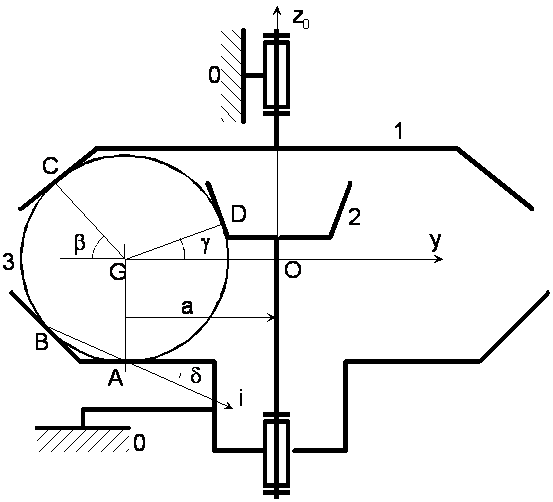
\includegraphics[width=\textwidth]{png/fig1}
\end{center}
\end{minipage}

\subparagraph{}
\textit{Trouver l’axe instantané de rotation du mouvement (axe central) de \textbf{3} par rapport à \textbf{0}. Il faudra justifier. Cet axe instantané de rotation est-il de direction fixe dans \textbf{0} ?}
\ifthenelse{\boolean{prof}}{%
\begin{corrige}
La condition de roulement sans glissement au point $A$ se traduit par $\vectv{A}{3}{0} =\vect{0}$.

La condition de roulement sans glissement au point $B$ se traduit par $\vectv{B}{3}{0} =\vect{0}$.

$A$ et $B$ sont donc des points où la norme du vecteur vitesse est minimale. Ce sont donc des points centraux. La droite $(AB)$ est donc un axe central. En conséquence, $\forall P \in (AB)$, alors, $\vectv{P}{3}{0}=\vect{0}$. 

Les points de contact $A$ et $B$ étant mobiles, la droite $(AB)$ n'a donc pas une direction fixe dans $\mathcal{R}_0$.
\end{corrige}
}{%
}


\subparagraph{}
\textit{Justifier l’écriture du vecteur $\vecto{3}{0} = \omega \vect{i}$ (avec $\omega$ composante scalaire du vecteur $\vecto{3}{0}$).}
\ifthenelse{\boolean{prof}}{%
\begin{corrige}
L'axe central étant de même direction que la résultante du torseur, on a donc nécessairement $\vecto{3}{0} = \omega \vect{i}$.
\end{corrige}
}{%
}

\subparagraph{}
\textit{Exprimer la relation entre $\dot{\psi}$ et $\omega$ issue du roulement sans glissement en $C$. On utilisera comme base de projection la base associée au repère $\mathcal{R}$.}
\ifthenelse{\boolean{prof}}{%
\begin{corrige}
D'après la relation de roulement sans glissement au point $C$ on a $\vectv{C}{3}{1} =\vect{0}$.
En conséquences, $\vectv{C}{3}{1} = \vectv{C}{3}{0} + \vectv{C}{0}{1}= \vectv{C}{3}{0} - \vectv{C}{1}{0} =\vect{0}$.

D'une part, calculons $\vectv{C}{3}{0}$ :
\begin{eqnarray*}
\vectv{C}{3}{0} &=&  \vectv{A}{3}{0} + \vect{CA}\wedge \vecto{3}{0} \\
& = & \left( R\cos\beta\vect{y} - R\left(1+\sin\beta\right) \vect{z_0}\right)\wedge\omega\vect{i}\\
& = & \left( R\cos\beta\vect{y} - R\left(1+\sin\beta\right) \vect{z_0}\right)\wedge\omega\left(\cos\delta\vect{y} - \sin\delta\vect{z_0} \right)\\
& = & -R\omega\cos\beta\sin\delta\vect{x} + R\omega\left(1+\sin\beta\right)\cos\delta\vect{x} 
\end{eqnarray*}

D'une part, calculons $\vectv{C}{1}{0}$ :
\begin{eqnarray*}
\vectv{C}{1}{0} &=&  \vectv{O}{3}{0} + \vect{CO}\wedge \vecto{1}{0} \\
& = & \left(\left(R\cos\beta +a\right)\vect{y} -R\sin\beta \vect{z_0}\right)\wedge \dot{\psi}\vect{z_0}\\
& = & \dot{\psi}\left(R\cos\beta +a\right)\vect{x}
\end{eqnarray*}

Au final, 
$$
\vectv{C}{3}{1} =\vect{0} \Longleftrightarrow -R\omega\cos\beta\sin\delta\vect{x} + R\omega\left(1+\sin\beta\right)\cos\delta\vect{x}  - \dot{\psi}\left(R\cos\beta +a\right)\vect{x} = \vect{0}
$$
Et donc :
$$
-R\omega\cos\beta\sin\delta + R\omega\left(1+\sin\beta\right)\cos\delta - \dot{\psi}\left(R\cos\beta +a\right) = 0
$$

\end{corrige}
}{%
}


\subparagraph{}
\textit{Exprimer la relation entre $\dot{\theta}$ et $\omega$ issue du roulement sans glissement en $D$. On utilisera comme base de projection la base associée au repère $\mathcal{R}$.}
\ifthenelse{\boolean{prof}}{%
\begin{corrige}

D'après la relation de roulement sans glissement au point $D$ on a $\vectv{D}{2}{3} =\vect{0}$.
En conséquences, $\vectv{D}{2}{3} = \vectv{D}{2}{0} + \vectv{D}{0}{3}= \vectv{D}{2}{0} - \vectv{D}{3}{0} =\vect{0}$.

D'une part, calculons $\vectv{D}{3}{0}$ :
\begin{eqnarray*}
\vectv{D}{3}{0} &=&  \vectv{A}{3}{0} + \vect{DA}\wedge \vecto{3}{0} \\
& = & \left( -R\cos\beta\gamma{y} - R\left(1+\sin\gamma\right) \vect{z_0}\right)\wedge\omega\vect{i}\\
& = & \left( -R\cos\beta\gamma{y} - R\left(1+\sin\gamma\right) \vect{z_0}\right))\wedge\omega\left(\cos\delta\vect{y} - \sin\delta\vect{z_0} \right)\\
& = &R\omega\cos\gamma\sin\delta\vect{x} + R\omega\left(1+\sin\gamma\right)\cos\delta\vect{x} 
\end{eqnarray*}

D'une part, calculons $\vectv{D}{2}{0}$ :
\begin{eqnarray*}
\vectv{D}{2}{0} &=&  \vectv{O}{2}{0} + \vect{DO}\wedge \vecto{2}{0} \\
& = & \left(\left(-R\cos\gamma -a\right)\vect{y} -R\sin\delta \vect{z_0}\right)\wedge \dot{\theta}\vect{z_0}\\
& = & \dot{\theta}\left(a-R\cos\gamma \right)\vect{x}
\end{eqnarray*}

Au final, 
$$
\vectv{D}{2}{0} =\vect{0} \Longleftrightarrow \dot{\theta}\left(a-R\cos\gamma \right)\vect{x} -  
R\omega\cos\gamma\sin\delta\vect{x} - R\omega\left(1+\sin\gamma\right)\cos\delta\vect{x}= \vect{0}
$$
Et donc :
$$
\dot{\theta}\left(a-R\cos\gamma \right) -  
R\omega\cos\gamma\sin\delta - R\omega\left(1+\sin\gamma\right)\cos\delta= 0
$$
\end{corrige}
}{%
}


\subparagraph{}
\textit{Déduire des deux réponses précédentes le rapport de réduction  $\dfrac{\dot{\theta}}{\dot{\psi}}$. }
\ifthenelse{\boolean{prof}}{%
\begin{corrige}
On a vu que :
\begin{eqnarray*}
-R\omega\cos\beta\sin\delta + R\omega\left(1+\sin\beta\right)\cos\delta - \dot{\psi}\left(R\cos\beta +a\right) = 0 
\Longleftrightarrow 
\dot{\psi}\left(R\cos\beta +a\right) = R\omega\left(-\cos\beta\sin\delta + \left(1+\sin\beta\right)\cos\delta \right) \\
\dot{\theta}\left(a-R\cos\gamma \right) - R\omega\cos\gamma\sin\delta - R\omega\left(1+\sin\gamma\right)\cos\delta= 0
\Longleftrightarrow 
\dot{\theta}\left(a-R\cos\gamma \right) = R\omega\left( \cos\gamma\sin\delta + \left(1+\sin\gamma\right)\cos\delta\right)
\end{eqnarray*}

En conséquence : 
$$
\dfrac{\dot{\theta}}{\dot{\psi}} = \dfrac{ R\omega\left( \cos\gamma\sin\delta + \left(1+\sin\gamma\right)\cos\delta\right)}{ R\omega\left(-\cos\beta\sin\delta + \left(1+\sin\beta\right)\cos\delta \right)}\cdot\dfrac{\left(R\cos\beta +a\right)}{\left(a-R\cos\gamma \right)}
$$

$$
\Longleftrightarrow \dfrac{\dot{\theta}}{\dot{\psi}} = \dfrac{ \cos\gamma\sin\delta + \cos\delta +\sin\gamma\cos\delta}{ -\cos\beta\sin\delta + \cos\delta+\sin\beta\cos\delta }\cdot\dfrac{\left(R\cos\beta +a\right)}{\left(a-R\cos\gamma \right)}
$$

$$
\Longleftrightarrow \dfrac{\dot{\theta}}{\dot{\psi}} = \dfrac{ \sin\left(\gamma+\delta \right) + \cos\delta }{\sin\left( \beta - \delta\right)+\cos\delta}\cdot\dfrac{\left(R\cos\beta +a\right)}{\left(a-R\cos\gamma \right)}
$$
\end{corrige}
}{%
}






\end{document}
